\section{Results}\label{sec:short_results}

\subsection{When does posterior integration matter?}

Figure~\ref{fig:short_mechanism} summarizes the synthetic mechanism experiment. The PI--PM difference grows when historical information is weak, volatility is high, maturity is long, little of the arithmetic average has already been fixed, and the option-pricing function is strongly curved in volatility. Across the full synthetic experiment, the maximum absolute PI--PM difference is 0.1384 on a normalized \$100 forward, and the largest cell-level 99th percentile is 0.1271. These values are economically nontrivial relative to the much smaller differences observed in the empirical WTI baseline.

The second-order approximation in Equation~\eqref{eq:short_taylor} closely tracks the simulated PI--PM difference. Across synthetic cells, the correlation between the cell-level mean gap and the curvature--variance approximation is 0.9995. In the most adverse cells, through-origin slopes are close to one. The synthetic evidence therefore supports a simple mechanism: posterior integration changes the point price when posterior variance and volatility curvature are simultaneously large.

Partial fixing generally reduces the integration correction because less of the payoff remains exposed to future volatility as the monthly average becomes known. The relationship need not be monotone at every intermediate state, however. In Panel C, the 252-day case initially rises before declining because partial fixing changes both remaining volatility exposure and the local curvature of the option-pricing function. The overall tendency is downward as the average approaches full fixation.

\begin{figure*}[t]
\centering
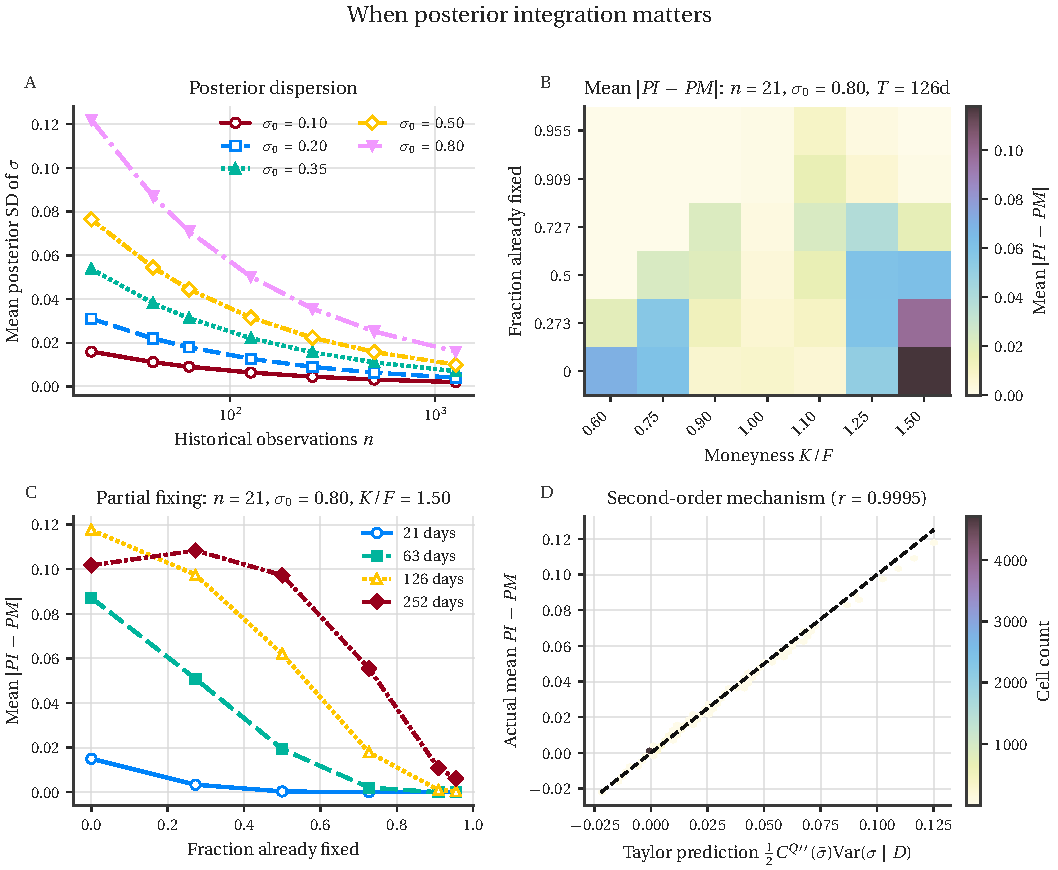
\includegraphics[width=\textwidth]{figures/publication/fig01_mechanism_map.pdf}
\caption{Posterior integration across synthetic WTI-like states. Panel A shows posterior dispersion against historical sample size. Panels B and C show how the absolute PI--PM difference varies with moneyness and the fraction of the averaging period already fixed. Panel D compares cell-level mean PI--PM differences with the corresponding second-order approximation in Equation~\eqref{eq:short_taylor}; the correlation is 0.9995. The color bar labeled \textit{Cell count} records how many synthetic scenario cells fall in each hexagonal bin of Panel D.}
\label{fig:short_mechanism}
\end{figure*}

\subsection{WTI point-price correction versus parameter uncertainty}

The October-2026 baseline contains 310 contract-date observations over 12 eligible valuation dates. Table~\ref{tab:short_october} reports the main Bayesian comparison. Posterior-integrated and posterior-mean plug-in prices have nearly identical market-pricing errors: RMSE is 0.5177 for PI and 0.5183 for PM. The mean absolute difference between the two prices is only 0.000745.

That near equality does not imply that uncertainty in the theoretical option value is negligible. The mean width of the central 95\% posterior interval for the model price is 0.2733, approximately 367 times the mean absolute PI--PM difference. The two quantities answer different questions. PI--PM measures how nonlinear averaging changes the posterior expectation of the option value; the interval width measures the dispersion of theoretical prices induced by uncertainty about volatility.

\begin{table}[t]
\centering
\caption{October-2026 WTI APO pricing and posterior price uncertainty. Pricing error is model price minus settlement price. All price quantities and errors are in U.S. dollars per barrel.}\label{tab:short_october}
\begin{tabular}{lrr}
\toprule
Quantity & $N$ & Value \\
\midrule
PI RMSE & 310 & 0.5177 \\
PM plug-in RMSE & 310 & 0.5183 \\
Mean $|PI-PM|$ & 310 & 0.000745 \\
Mean 95\% posterior price-interval width & 310 & 0.2733 \\
\bottomrule
\end{tabular}
\end{table}

The common pricing bias also points away from posterior integration as the main empirical margin. Both historical-volatility prices understate settlement values on average in the October baseline, and PI and PM differ by less than one tenth of a cent per barrel on average. A different volatility input therefore has much more room to affect pricing performance than a more exact integration of this relatively concentrated posterior.

\subsection{Historical versus option-implied volatility}

Table~\ref{tab:short_forward} reports the central out-of-sample comparison. On the same 2,381 contract-date observations, the long-window historical posterior-integrated benchmark has MAE 2.6187 and RMSE 3.4090. The best of the pre-specified rolling-window comparisons, based on the most recent 63 returns, has still larger errors, with MAE 4.5201 and RMSE 5.6465. The horizon-matched GARCH(1,1) benchmark produces MAE 2.6730 and RMSE 3.4441, close to the long-window historical benchmark.

By contrast, the previous-day APO implied-volatility smile has MAE 0.1075 and RMSE 0.1594. The expanding earlier-date smile produces similarly small errors, 0.1088 and 0.1725. The difference is present in every admitted expiry rather than being produced by one maturity. Valuation-date cluster bootstrap intervals for the error differences also remain well below zero across the seven expiries, as shown in Figure~\ref{fig:short_forward_bootstrap}.

\begin{table*}[t]
\centering
\caption{Historical-volatility and prior option-implied volatility benchmarks. Panel A uses the same 2,381 out-of-sample contract-date observations over 15 target dates. Panel B restricts the comparison to observations for which the same contract has a strictly prior implied volatility. Historical PI is the canonical Monte Carlo posterior-integrated price; scalar historical, GARCH, and implied-volatility inputs are repriced under the same Curran approximation. MAE and RMSE are in U.S. dollars per barrel.}\label{tab:short_forward}

\textit{Panel A: main out-of-sample comparison}\\[2pt]
\begin{tabular}{lrrrr}
\toprule
Volatility input & $N$ & Dates & MAE & RMSE\\
\midrule
Historical PI & 2,381 & 15 & 2.6187 & 3.4090\\
Rolling 63 returns & 2,381 & 15 & 4.5201 & 5.6465\\
Horizon-matched GARCH(1,1) & 2,381 & 15 & 2.6730 & 3.4441\\
Previous-day APO implied-volatility smile & 2,381 & 15 & 0.1075 & 0.1594\\
\bottomrule
\end{tabular}

\vspace{5pt}
\textit{Panel B: same-contract lagged-IV benchmark}\\[2pt]
\begin{tabular}{lrrrr}
\toprule
Volatility input & $N$ & Dates & MAE & RMSE\\
\midrule
Historical PI & 2,366 & 15 & 2.6279 & 3.4173\\
Same-contract lagged IV & 2,366 & 15 & 0.0992 & 0.1403\\
Previous-day fitted APO smile & 2,366 & 15 & 0.1074 & 0.1594\\
\bottomrule
\end{tabular}
\end{table*}

The historical comparisons address two natural alternatives. First, the difference is not reproduced by simply shortening the return window or by using an exponentially weighted historical estimate; the complete set of rolling-window and EWMA results is reported in Online Supplement Section S1 and Table S1. Second, allowing conditional heteroskedasticity and forecasting variance over the remaining fixing horizon does not materially close the pooled gap: GARCH remains near the long-window historical benchmark.

Panel B addresses a different alternative. On the exact common sample, carrying the same contract's latest prior implied volatility forward has lower pooled MAE and RMSE than fitting the previous-day smile. This is a descriptive ranking rather than evidence that lagged IV is generally superior to a fitted smile. Its role is to show that the large historical-versus-option-implied difference does not require a flexible cross-sectional implied-volatility function.

\begin{figure*}[t]
\centering
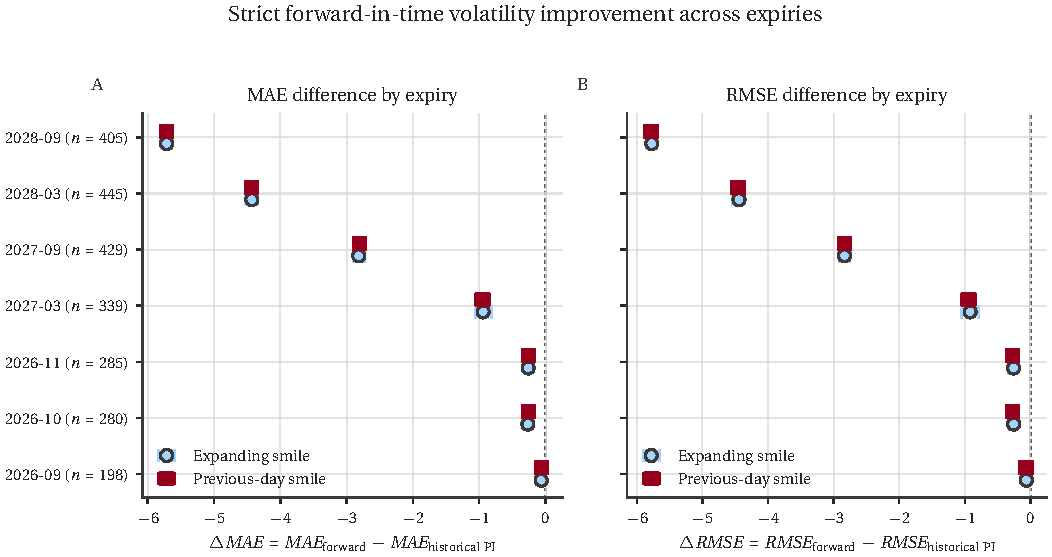
\includegraphics[width=\textwidth]{figures/publication/fig03_forward_q_cluster_bootstrap.pdf}
\caption{Out-of-sample pricing-error differences by APO expiry. Points compare the earlier-date APO implied-volatility specifications with the historical posterior-integrated benchmark; negative values indicate lower error for the implied-volatility specification. Horizontal bars are 95\% percentile intervals from valuation-date cluster bootstrap resampling. All implied-volatility inputs are estimated only from dates earlier than the target date.}
\label{fig:short_forward_bootstrap}
\end{figure*}

The economic interpretation should remain conditional on the model. Historical volatility and option-implied volatility are not two estimators of an identical observable object. The latter can incorporate risk premia and can also compensate for omitted stochastic volatility, jumps, futures-curve dynamics, and market-marking effects. The out-of-sample result therefore establishes a difference in pricing information under the maintained model, not a structural decomposition of the physical and risk-neutral volatility processes.

\subsection{Cross-instrument validation using vanilla-WTI options}

The independent vanilla-WTI experiment moves the implied-volatility source outside the APO market. Table~\ref{tab:short_lo} reports the exact common sample of 253 October-2026 APO contract-dates over 10 valuation dates. Historical-volatility posterior integration has MAE 0.4464 and RMSE 0.5562. A previous-day vanilla-WTI implied-volatility specification based on LO options lowers these errors to 0.1559 and 0.2599. The corresponding previous-day APO implied-volatility smile has MAE 0.1676 and RMSE 0.2686.

\begin{table}[t]
\centering
\caption{Cross-instrument validation on 253 October-2026 APO contract-dates within observed prior LO moneyness support. Historical PI is the canonical Monte Carlo posterior-integrated price; the vanilla-WTI and APO implied-volatility inputs are repriced with the deterministic Curran approximation. All implied-volatility inputs use only earlier-date option information. MAE and RMSE are in U.S. dollars per barrel.}\label{tab:short_lo}
\begin{tabular}{lrr}
\toprule
Volatility input & MAE & RMSE\\
\midrule
Historical PI & 0.4464 & 0.5562\\
Previous-day vanilla-WTI IV & 0.1559 & 0.2599\\
Previous-day APO IV & 0.1676 & 0.2686\\
\bottomrule
\end{tabular}
\end{table}

Valuation-date cluster bootstrap intervals preserve the improvement of the external LO specification relative to historical volatility. The external and APO-implied results are much closer to one another, and their difference is not uniformly distinguishable across MAE and RMSE. The relevant conclusion is therefore not that LO is superior to APO-implied volatility. It is that the pricing improvement associated with prior option-implied volatility persists when the information is obtained from another WTI option family.

Taken together, the results separate the two empirical margins. Posterior integration can matter when posterior variance meets option-price curvature, and the synthetic experiment identifies those states clearly. In the observed WTI sample, however, the PI--PM point-price effect is small. The substantially larger empirical difference comes from the volatility information supplied to the pricing model.
